\section{Automotora Pycar}

La automotora PyCar requiere generar información importante con respecto a sus ventas.
Principalmente requiere realizar un análisis sobre el desempeño de sus vendedores así como también sobre la evolución de las ventas que se van realizando.

Para lograr este propósito, PyCar tiene almacenado en un archivo del tipo \texttt{productos.txt} la información del precio de los automóviles que tiene a la venta. Cada producto viene especificado por la marca del automóvil, el modelo y el precio de venta. Por otro lado, PyCar almacena en un archivo del tipo \texttt{ventas.txt}, cada una de las transacciones realizadas por concepto de la venta
de un automóvil (ordenadas por fecha), esta información cuenta con el día de la venta, la hora en que se ha realizado, el modelo del automóvil, la marca del mismo y el código del vendedor que ha realizado la transaccion. 

\paragraph{Nota:} los archivos sonejemplos, su programa debe funcionar para toda la cantidad de automóviles que puede tener la automotora y para todas las ventas que se han realizado durante el año 2014.

\begin{figure}[h]
    \centering
    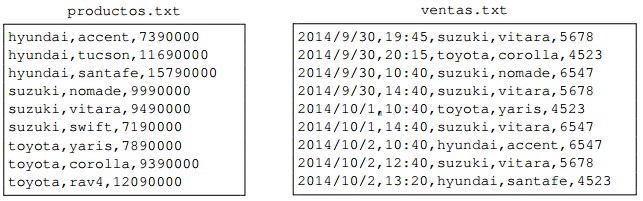
\includegraphics[scale=0.8]{Imagenes/autos.png}
\end{figure}

Con el fin de ayudar a PyCar en sus requerimientos, Ud. debe realizar lo siguiente:

\begin{itemize}
    \item[a)] Desarrolle la función \texttt{precios(archivo)} que recibe el nombre del archivo con la información de los productos y retorne un diccionario, donde la llave sea el modelo del automóvil y el valor sea el precio del mismo.
    
\begin{lstlisting}[style=consola]
>>> precios('productos.txt')
{'rav4': 12090000, 'corolla': 9390000, 'accent': 7390000, 'nomade': 9990000,
'yaris': 7890000, 'tucson': 11690000, 'santafe': 15790000, 'swift': 7190000,
'vitara': 9490000}
\end{lstlisting}

    \item[b)] Desarrolle la función \texttt{total\_ventas\_mes(codigo, mes, archivo1, archivo2)} que recibe el código de un vendedor, un mes en particular, el nombre del archivo con la información de los productos y el nombre del archivo con la información de las ventas y retorne el total de ventas que ha realizado el vendedor en ese mes.
    
\begin{lstlisting}[style=consola]
>>> total_ventas_mes(4523, 10, 'productos.txt', 'ventas.txt')
23680000
\end{lstlisting}
    \item[c)] Desarrolle la función \texttt{venta\_diaria(archivo1,archivo2)} que recibe el nombre del archivo con la información de los productos y el nombre del archivo con la información de las ventas y genere el archivo \texttt{venta\_diaria.txt} indicando la venta total que se ha realizado por día.
\begin{lstlisting}[style=consola]
>>> venta_diaria('productos.txt','ventas.txt')
>>>
\end{lstlisting}
\begin{figure}[h]
\centering
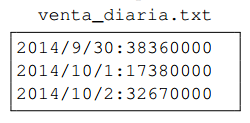
\includegraphics[scale=0.7]{Imagenes/ventadiaria.png}
\end{figure}
\end{itemize}
